\subsection{Unlocking RF Magic: The Three Key Calibration Loads!}

What three test loads are used to calibrate an RF vector network analyzer? 

\begin{tcolorbox}[colback=gray!10, colframe=black, title=E4B05]
     What three test loads are used to calibrate an RF vector network analyzer?  
\begin{enumerate}[label=\Alph*.]
    \item 50 ohms, 75 ohms, and 90 ohms
    \item \textbf{Short circuit, open circuit, and 50 ohms}
    \item Short circuit, open circuit, and resonant circuit
    \item 50 ohms through 1/8 wavelength, 1/4 wavelength, and 1/2 wavelength of coaxial cable
\end{enumerate} \end{tcolorbox}

\subsubsection{Understanding RF Vector Network Analyzers}

An RF vector network analyzer (VNA) is a sophisticated instrument used to measure the electromagnetic properties of radio frequency devices. Calibration of a VNA is crucial for accurate measurements and involves using known test loads to ensure that the system compensates for any losses or reflections present in the measurement setup.

In this context, the three test loads typically employed for calibration are:

1. \textbf{Short Circuit} - This provides a reference for the situation where the end of the transmission line is connected directly to ground, resulting in very low impedance.
2. \textbf{Open Circuit} - In this case, the transmission line does not connect to any load, providing a reference for a very high impedance condition.
3. \textbf{50 Ohms} - This is a standard impedance commonly used in RF applications, offering an intermediate reference that is essential for matching different components in real-world applications.

\subsubsection{Concepts Required for Understanding}

To grasp why these specific test loads are used, it is important to understand the concepts of impedance, reflection coefficients, and S-parameters:

- \textbf{Impedance (Z)} describes how much resistance an electrical component poses against the flow of alternating current. In RF applications, the standard impedance is usually 50 ohms.
- \textbf{Reflection Coefficient ($ \Gamma $ )} measures how much of an electromagnetic wave is reflected back when it encounters a load with a different impedance compared to the transmission line.
- \textbf{S-parameters (Scattering parameters)} are measures that describe the input-output relationship of a linear electrical network and are fundamental in characterizing the properties of RF networks.

By using these three calibration loads, the VNA can characterize how devices reflect and transmit signals, allowing engineers to design more effective RF circuits.

\subsubsection{Visualization}

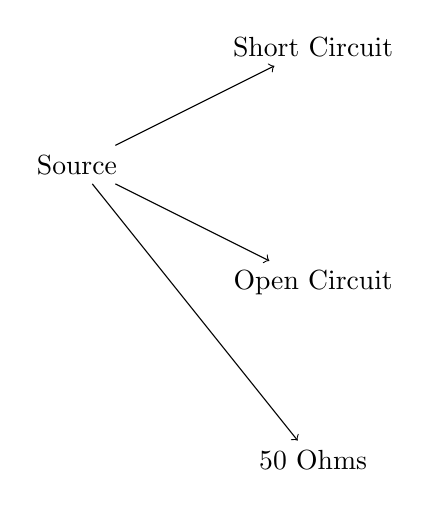
\begin{tikzpicture}[scale=1.5]
    \node (source) at (0, 0) {Source};
    \node (short) at (2, 1) {Short Circuit};
    \node (open) at (2, -1) {Open Circuit};
    \node (load) at (2, -2.5) {50 Ohms};
    
    \draw[->] (source) -- (short);
    \draw[->] (source) -- (open);
    \draw[->] (source) -- (load);
\end{tikzpicture}

This diagram represents the flow of signals from the source to the three different types of loads that are used for calibrating the RF vector network analyzer. It highlights the relationship between the source and the test loads which is critical in ensuring accurate measurement and analysis.
